% !TEX root = main.tex
\chapter{System overview}\label{cha:systemOverview}
This chapter provides the reader with a brief overview of the whole collimator system used in the \abbrLHC at \abbrCERN as well as a more detailed description of the rotational stage, which is the device in focus in this thesis.

\section{Crystal collimators}
A collimator is a specially designed device, built to interfere with the beam and clean it from surrounding halo particles. To be able to meet the future demand of higher energy levels, a more efficient collmator is being devloped at CERN. This new collimator will utilze a crystaline solid to extract particles from the beam. The collimator consists of a T-shape structure containg two movable linear axes and one rotational stage. Each linear axis is driven by a stepping motor, labeled as \emph{M1} and \emph{M2} in Figure~\ref{fig:collimator-side}, seperately controlled in open-loop by an individual drive unit. The motor driving the vertical axis, \emph{M1}, is used to move a piece of beampipe down inside the T-shape, giving access to the horizontal axis, driven by \emph{M2}, to move the rotaional stage (including the crystal) into the beampipe to interfere with the beam. The directions of the crystal's linear and rotational movement are indicated by the arrows in Figure~\ref{fig:collimator-top}.
During operation, Physicists will drive the crystal close to the beam, enter it with an angle and rotate it slightly (in the range of \unit{10}{\milli\rad}) until the channeling effect is detected. Channeled particles will then be bent off the bem core and abosorbed further down the beam pipe.

\begin{figure}[tpb]
 \centering %crop: left bottom right top
 \subfloat[][\label{fig:collimator-side}Collimator from side]{
 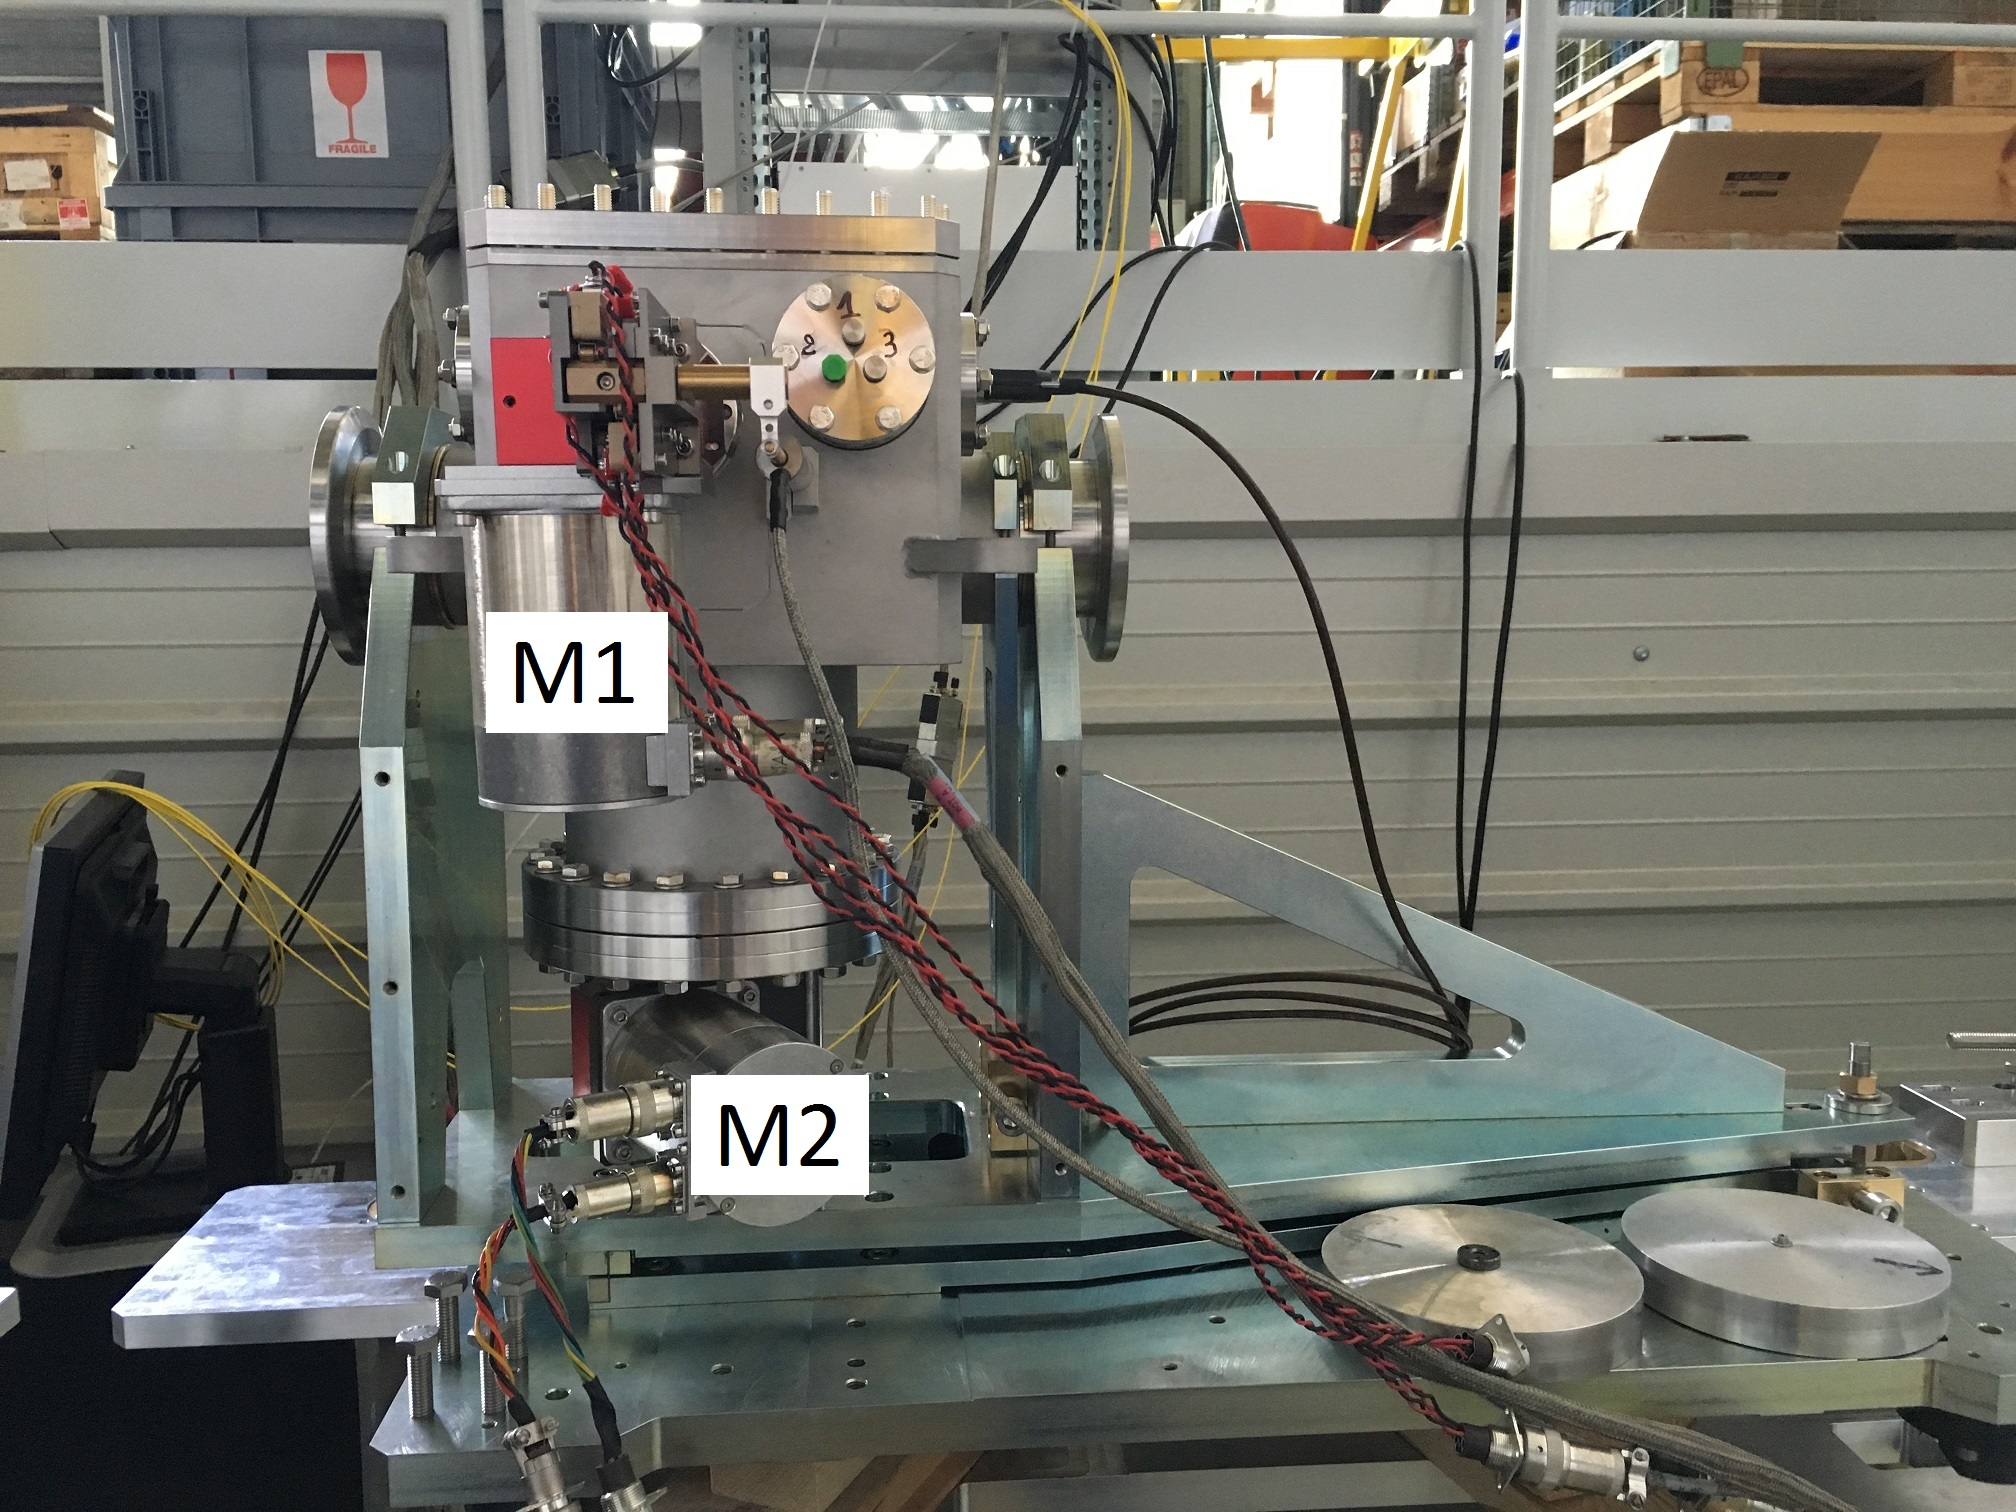
\includegraphics[width=0.5\textwidth, trim=10cm 12cm 50cm 7cm, clip=true]{fig/collimator-side}}
 \qquad
 \subfloat[][\label{fig:collimator-top}Collimator from top]{
 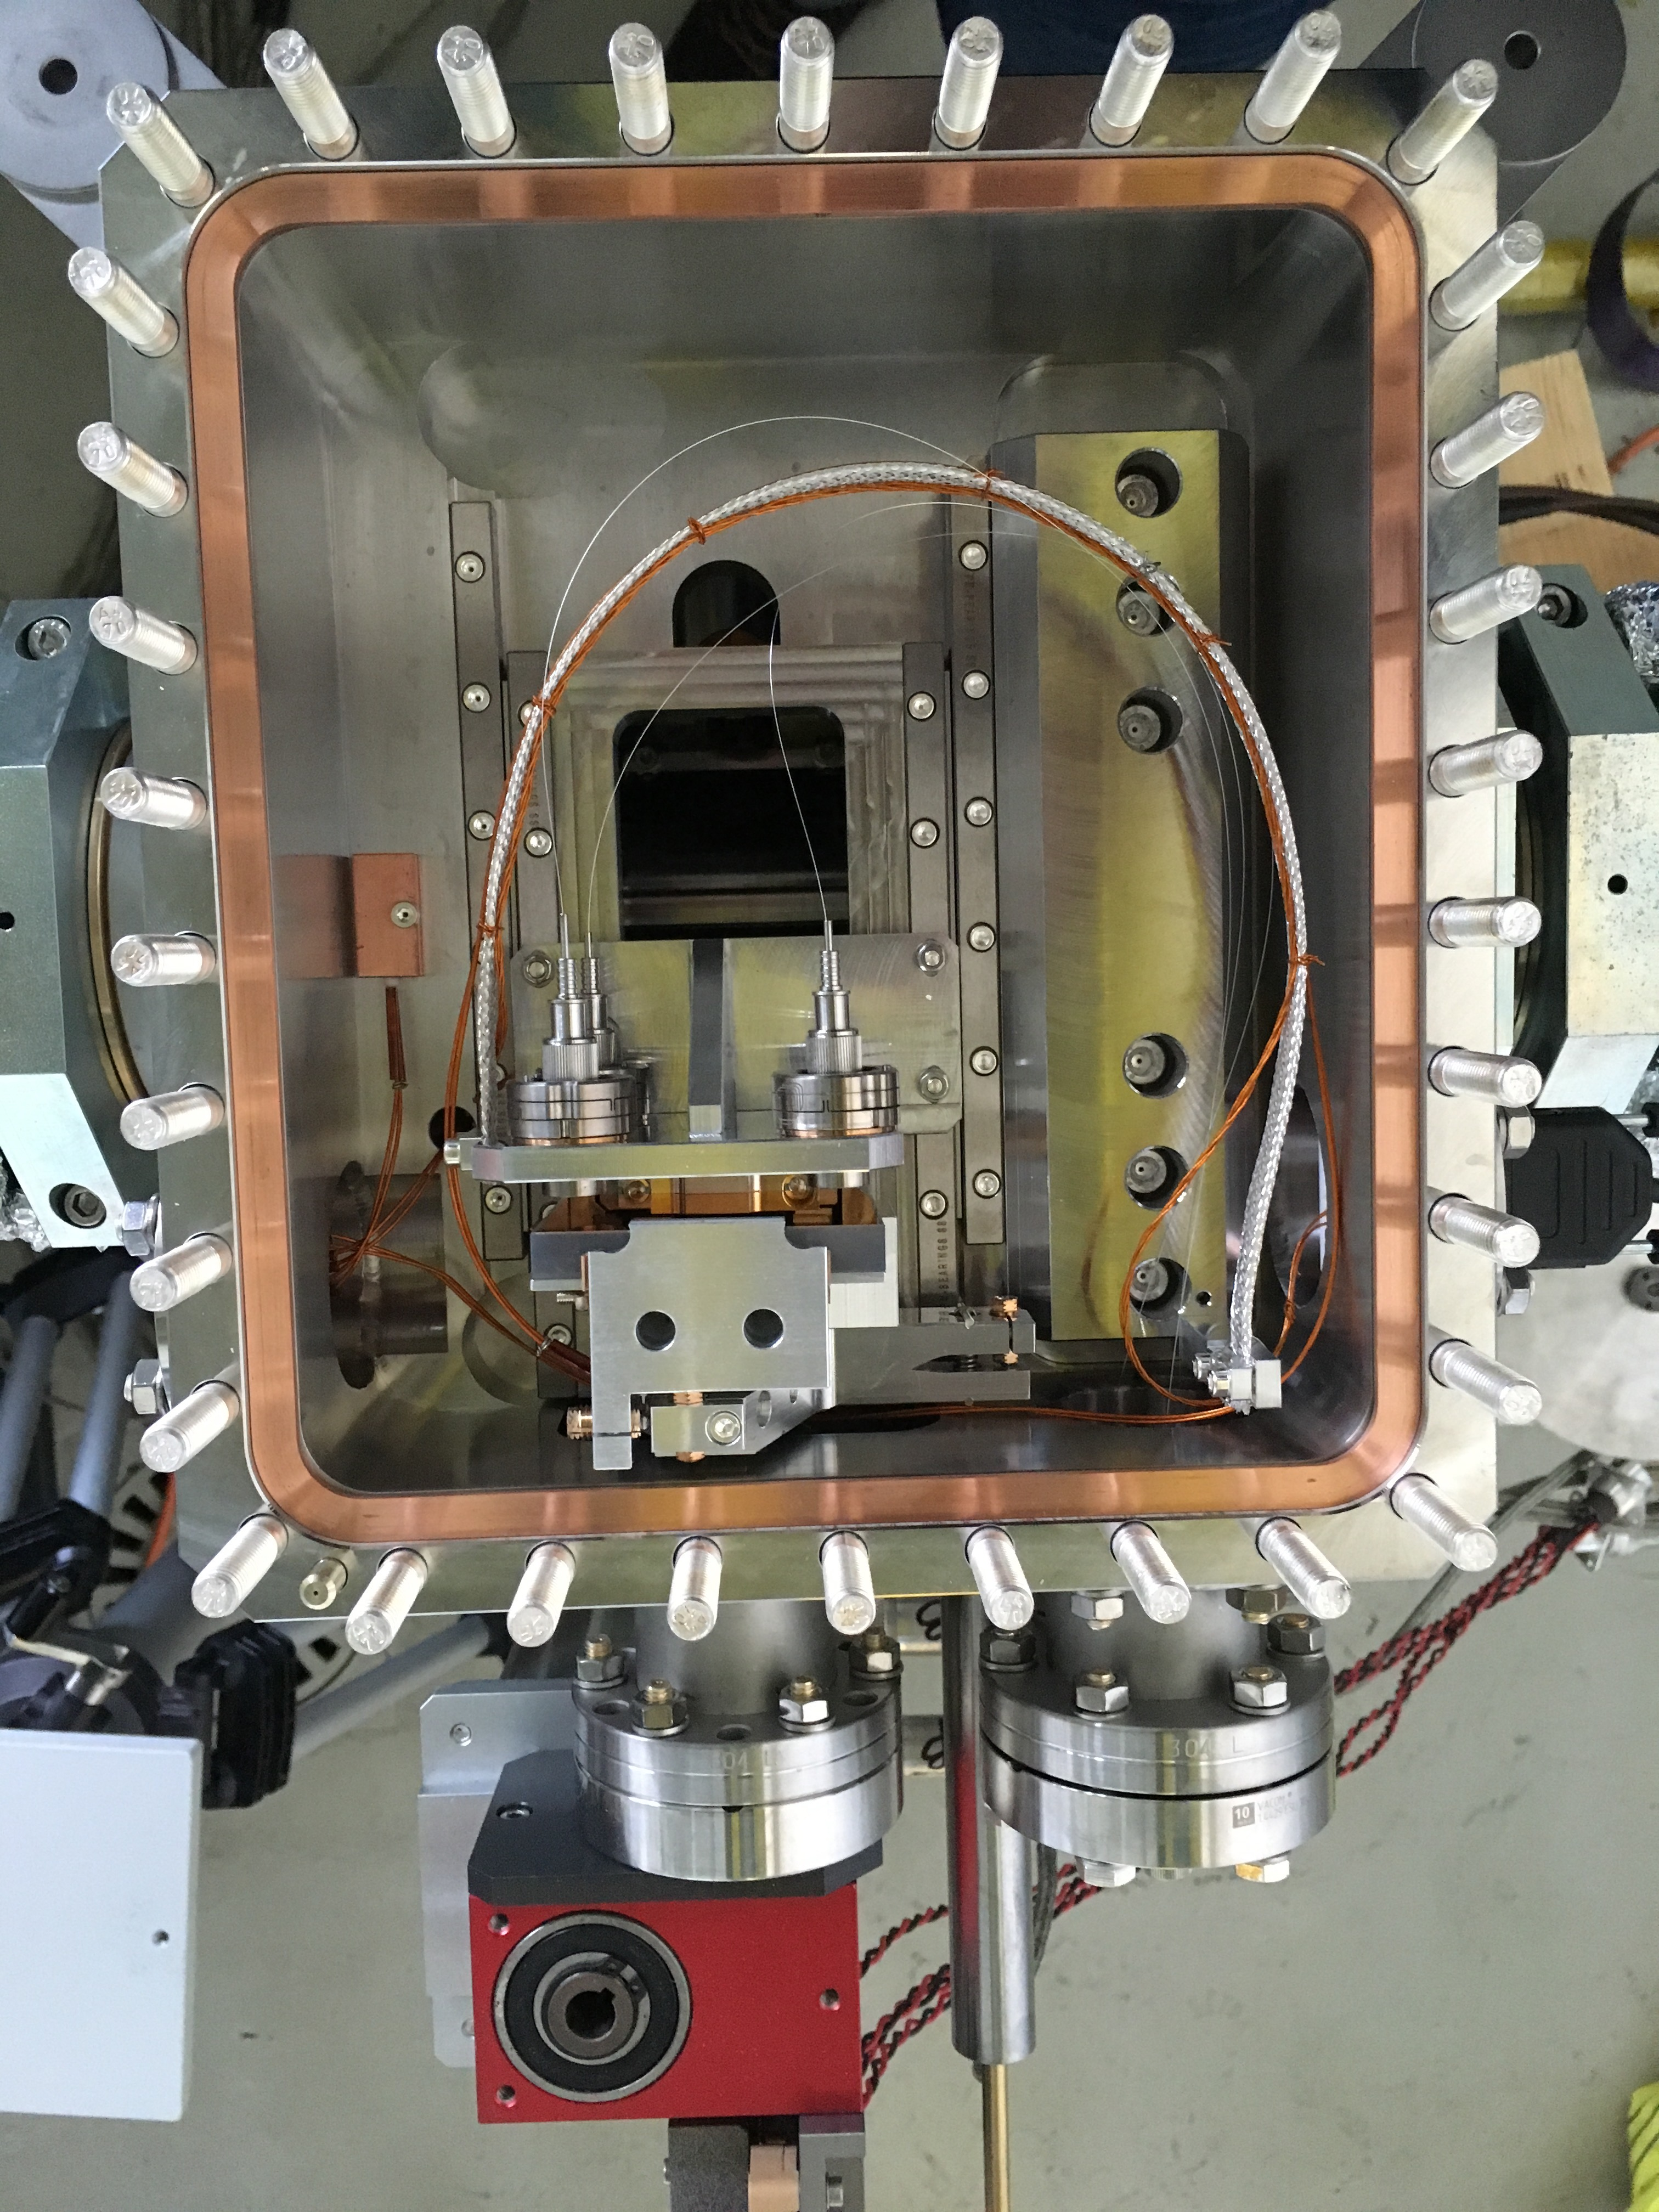
\includegraphics[width=0.4\textwidth, trim=0cm 0cm 0cm 0cm, clip=true]{fig/collimator-top}}
 \caption{\label{fig:collimator} Illustrates the collimator from the side (a) and the top (b).}
\end{figure}

\section{Rotational stage}
The rotational stage as shown in Figure? is composed by a monolitic structure, a prestressed piezo stack actuator and an interferometer measurement system. The flexure-hinge based structure, avoids sliding parts and thereby enhance precision by reducing the number of nonlinear effects (e.g. backlash and friction). A prestressed piezo stack actuator is exploited to generate the rotaional movement by interacting on a point 4mm away from the center of rotation, see Figure. This amplyfing structure gives the rotational stage a range of \unit{20}{\milli\rad}. For the measurement system, 3 interferometric heads are placed as in Figure ?, pointing towards a mirror mounted ontop of to the rotaional head, perpendicular to the plane of rotation. The setup allows for measurements of both the yaw and roll angle (the coordnate system is defined with respect to the beam). The yaw angle is used as feedback to the rotational stage control loop. The spring, depicted in Figure?, prestresses the \abbrPESA in order to enhace the overall stiffness of the stage as well as keeping the stackplates in place (the stack is nonglued to be sufficient in a radioactive area). This combinataion leads to an unmistaken resonsant structure, due to the characteristics of the \abbrPESA demanding in combination with the spring, demanding a properly designed controller. The system moving the crystal, i.e. the linear axis driven by \emph{M2} and the rotaional stage needs to be able to track reference trajectories at ramp rates of \unit{100}{\micro\radianpersecond} and reject external disturbances to maintain a maximum tracking error of $\pm$\unit{1}{\micro\rad}.

\section{Piezoelectric stack actuator}
The rotational stage uses a linear piezoelectric stack actuator to create the movement. It provides a displacement range from 0 to \unit{30}{\micro\meter}, corresponding to 0 and 150V, respectively. {\abbrPESA}s are made of many thin, stacked electroactive cheramic disks, electrically connected in parallell. This construction allows for an actuator that can exhibit the highest stiffness of all actuators designs but still with a high displacement range \cite{Piezo:2008}.

\subsection{Hysteresis effect}
The hysteresis effect is a nonlinear effect that is present during the operation of piezopelectric actuators. It occurs when the driving direction is reversed and origins from the polarization and the molecular effects in the piezoceramic. It depends on the amplitude of the applied voltage but also on the frequency of input signals \cite{Qingson:2016}. Figure~\ref{fig:hysteresis} illustrates the hysteresis effect. One can see how the same voltage value (e.g. 60V) corresponds to one angular position (\unit{5,2}{\micro\rad}) in one direction and another one in the opposite direction (\unit{7,2}{\micro\rad}).

\begin{figure}[h]
 \centering %crop: left bottom right top
 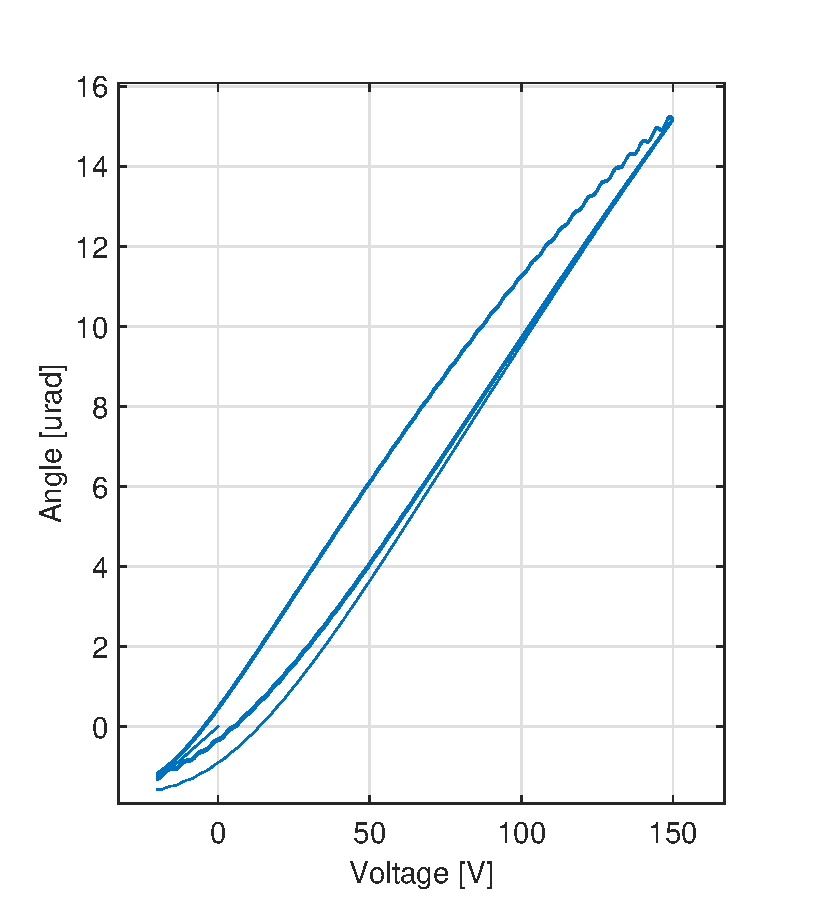
\includegraphics[width=0.5\textwidth]{fig/matlab/hysteresis.eps}
 \caption{\label{fig:hysteresis}Illustration of the hysteresis effect.}
\end{figure}

\subsection{Creep effect}
The creep effect is another nonlinear effect that is present during the operation of piezoelectric actuators. The effect is a slow elongation or contraction of the actuator displacement over time, with a constant driving signal and is caused by thermal effects in the piezoceramics. Figure~\ref{fig:creep} illustrates the creep effect. One can see how the rotainalstage slightly drifts in rotation after the applied negative step.

\begin{figure}[h]
 \centering %crop: left bottom right top
 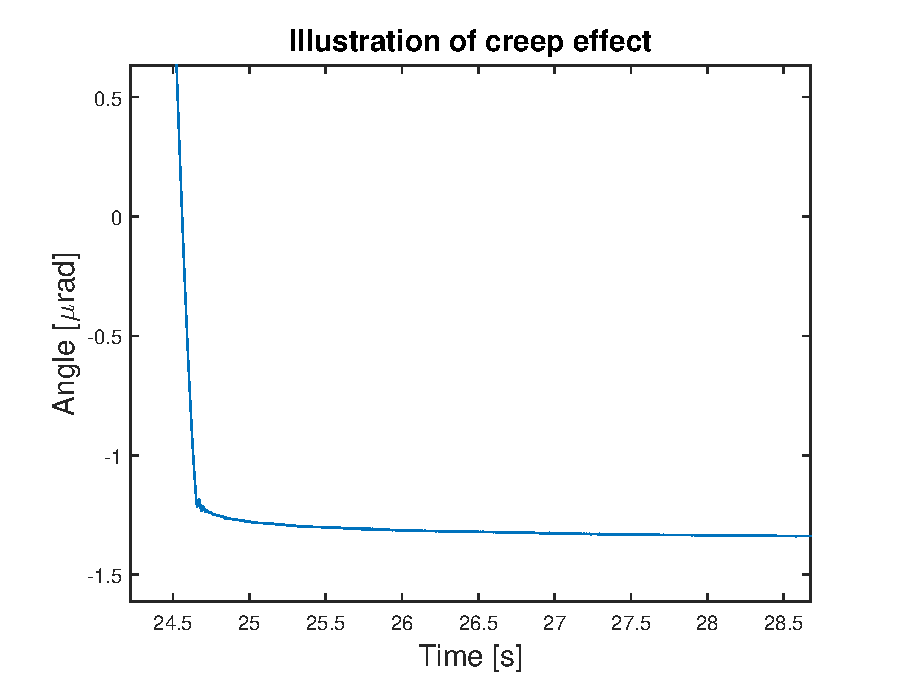
\includegraphics[width=0.5\textwidth]{fig/matlab/creep.eps}
 \caption{\label{fig:creep}Illustration of the creep effect. Note that the creep effect can last up to 10-15 minutes even if the plot only shows the development over 4 seconds.}
\end{figure}

\section{System identification}

\section{Present control loop}
The original controller for the rotaional stage is a PID controller which is used in combination with a pre-filter and a hysteresis compensator.
